%- - - - - - - - - - - - - - - - - - - - - - - - - - - - - - - - - SLIDE -
\begin{frame}
\frametitle{Complete Search}
\begin{block}{}
\begin{itemize}
	\bitem Estratégia baseada no princípio KISS (``Keep It Simple, Stupid'')
	\begin{itemize}
		\bitem Buscar os resultados evitando qualquer complexidade desnecessária.
	\end{itemize}
	\bitem O objetivo numa competição de programação é escrever um programa que resolva o problema dentro do tempo limite.
	\begin{itemize}
		\bitem Não importa se existe ou não uma solução mais eficiente.
	\end{itemize}
	\bitem A busca exaustiva faz uso do método trivial, de força bruta, todas as possíveis soluções são analisadas para encontrar a resposta.
	\bitem Essa técnica sempre deve ser a primeira a ser considerada.
	\begin{itemize}
		\bitem Caso funcione dentro do limite de tempo / memória, use-a! 
		\begin{itemize}
			\bitem Geralmente é fácil de codificar e debugar.
%			\bitem Mais tempo para trabalhar nos problemas difíceis. 
		\end{itemize}
	\end{itemize}
	\bitem Apenas alguns milhões de possíveis respostas para um problema? Itere em todas elas e encontre aquela que funciona.
\end{itemize}
\end{block}
\pause

\begin{block}{\tiny Cuidado!!}
Nem sempre é óbvio que a busca exaustiva pode ser usada.
\end{block}
\end{frame}

%- - - - - - - - - - - - - - - - - - - - - - - - - - - - - - - - - SLIDE -
\begin{frame}
\frametitle{Complete Search}

\begin{block}{}
\begin{itemize}
	\bitem Uma das técnicas de resolução de problemas mais importantes;
	\begin{itemize}
		\bitem Pode ser aplicada a uma grande gama de problemas quando as instâncias são pequenas os suficiente
		\bitem Ponto de partida para o desenvolvimento de outros algoritmos.
	\end{itemize}
	\bitem Competidor precisa saber:
	\begin{itemize}
		\bitem Gerar/testar: subconjuntos, permutações, ...
		\bitem Técnicas para reduzir o espaço de busca
		\bitem Estimar a complexidade no pior caso
	\end{itemize}
	\bitem Ajustes no código podem influenciar bastante no tempo de execução;
	\begin{itemize}
		\bitem Vale a pena implementar a mesma solução de formas diferentes.
	\end{itemize}
\end{itemize}	
\end{block}

\begin{block}{\tiny \#protip}
Quando não conseguir pensar em um jeito melhor de resolver o problema arrisque a solução por força bruta.
Caso exista um caso onde ela não é rápida o suficiente, mantenha a solução por perto e use-a para testar outras soluções nos casos menores.
\end{block}
\end{frame}

%- - - - - - - - - - - - - - - - - - - - - - - - - - - - - - - - - SLIDE -
\begin{frame}
\frametitle{Complete Search}
\begin{block}{Filtrar vs. Gerar }
Duas possíveis abordagens podem ser escolhidas quando fazendo uma busca exaustiva:
\begin{itemize}
	\bitem Filtragem -- Todas as possíveis soluções são geradas e depois examinadas para eliminar as inválidas.
	\bitem Geração -- Soluções construídas progressivamente, assim que uma inconsistência é detectada a solução é descartada.
\end{itemize}
\end{block}
\pause
\begin{block}{}
\begin{itemize}
	\bitem Candidato parcial (estado) -- parte de uma possível solução;
	\begin{itemize}
		\bitem Pode ser completado (através de um passo de extensão) de diferentes maneiras para gerar uma solução.
	\end{itemize}	
	\bitem Candidatos são os nós de uma árvore. Cada candidato parcial é pai dos candidatos que podem ser obtidos a partir dele em um passo de extensão.
\end{itemize}
\end{block}
\end{frame}

%- - - - - - - - - - - - - - - - - - - - - - - - - - - - - - - - - SLIDE -
\begin{frame}
\frametitle{Complete Search}
% TODO figura mostrando uma árvore..
\huge FIGURA ILUSTRANDO ARVORE
\end{frame}

%- - - - - - - - - - - - - - - - - - - - - - - - - - - - - - - - - SLIDE -
\begin{frame}
\frametitle{Complete Search}
\begin{block}{Problema: $n$ Queens}
\scriptsize
Colocar $n$ rainhas em um tabuleiro de xadrez $n\ x\ n$ de modo que uma rainha não ataque outra.
\end{block}
\pause
\begin{block}{Abordagens..}
\begin{itemize}[<+->]
	\bitem 1. Gerar $n$ pares $(x,y)$ e verificar se formam uma solução válida.
	\begin{itemize}
		\item[] $n^{2n}$ -- \textbf{\textcolor{red}{BAD!}}
	\end{itemize}
	\bitem \texttt{$Obs_1$.: Cada coluna deve ter exatamente uma rainha..}
	\bitem 2. Gerar as $n^n$ possíveis soluções e verificar se são válidas.
	\begin{itemize}
		\item[] \textbf{Melhorou, só que não!}
	\end{itemize}
	\bitem \texttt{$Obs_2$.: Cada linha também tem exatamente uma rainha..}
	\bitem 3. Gerar as $n!$ possíveis soluções e verificar se são válidas.
	\begin{itemize}
		\item[] \textbf{Hmm, parece ``bom''.. será que dá pra melhorar?}
	\end{itemize}
\end{itemize}
\end{block}
\end{frame}

%- - - - - - - - - - - - - - - - - - - - - - - - - - - - - - - - - SLIDE -
\begin{frame}
\frametitle{Complete Search}
\begin{block}{Problema: $n$ Queens}
\scriptsize
Colocar $n$ rainhas em um tabuleiro de xadrez $n\ x\ n$ de modo que uma rainha não ataque outra.
\end{block}

\begin{block}{Busca em profundidade, Backtracking}
\begin{itemize}[<+->]
	\bitem Podemos tentar adicionar as rainhas uma por uma, recursivamente, no tabuleiro.
	\bitem Explorando o fato de que é necessário colocar uma rainha por coluna, em cada passo da recursão basta escolher em qual linha na coluna atual colocar a rainha.
	\bitem Não faz sentido colocar uma rainha em uma posição que entra na zona de ataque de alguma das rainhas anteriormente colocadas.
	\bitem Continuamos tentando gerar as $n!$ permutações, mas agora só geramos aquelas que são válidas. \color{ccomments}{(filtrar vs. gerar)}
\end{itemize}
\end{block}
\end{frame}

%- - - - - - - - - - - - - - - - - - - - - - - - - - - - - - - - - SLIDE -
\begin{frame}
\frametitle{Complete Search}
\begin{block}{Problema: $n$ Queens}
\scriptsize
Colocar $n$ rainhas em um tabuleiro de xadrez $n\ x\ n$ de modo que uma rainha não ataque outra.
\end{block}

\begin{block}{Busca em profundidade, Backtracking}
\includefile{c++}{codes}{pseudonqueen.cpp}
\end{block}
\end{frame}

%- - - - - - - - - - - - - - - - - - - - - - - - - - - - - - - - - SLIDE -
\begin{frame}
\frametitle{Complete Search}

\begin{block}{Busca em profundidade, Backtracking}

\begin{itemize}
	\bitem Essa abordagem é um exemplo de uma busca em profundidade (DFS - \emph{Depth First Search})
	\begin{itemize}
		\bitem O algoritmo tenta iterar do topo ao fundo da árvore o mais rápido possível.
		\bitem Um vez que $k$ rainhas são colocadas no tabuleiro, apenas tabuleiros com mais rainhas são examinados.
	\end{itemize}
	\bitem O algoritmo busca na árvore de cima para baixo, analisando os candidatos parciais.
	\bitem Quando uma solução é encontrada ou uma inconsistência detectada, o mecanismo de \emph{backtracking} entra em ação
	\begin{itemize}
		\bitem O caminho que levou até aquela solução é percorrido ao contrário até que uma nova extensão possa ser gerada.
	\end{itemize}
\end{itemize}
\end{block}
\end{frame}

%- - - - - - - - - - - - - - - - - - - - - - - - - - - - - - - - - SLIDE -
\begin{frame}
\frametitle{Complete Search}
	\begin{center}
		\begin{figure}
			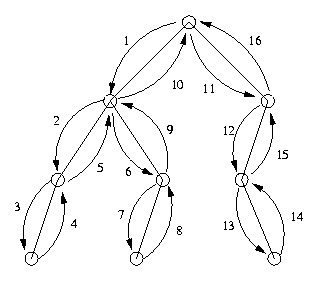
\includegraphics[width=.52\textwidth]{figuras/dfs.png}
			\caption{USACO}
		\end{figure}
	\end{center}
\end{frame}

%- - - - - - - - - - - - - - - - - - - - - - - - - - - - - - - - - SLIDE -
\begin{frame}
\frametitle{Complete Search}

\begin{block}{Busca em profundidade, Backtracking - Complexidade}

\begin{itemize}
	\bitem Seja $d$ o número de decisões que devem ser feitas 
	\begin{itemize}
		\item[] \scriptsize{No caso das $n$-rainhas $d=n$, o nro. de colunas que devemos preencher.}
	\end{itemize}
	\bitem Seja $C$ a quantidade de escolhas para cada decisão
	\begin{itemize}
		\item[] \scriptsize{No caso das $n$-rainhas $C=n$, já que qualquer uma das linhas pode ser escolhida.}
	\end{itemize}
	\bitem No pior caso, a busca leva tempo $O(C^d)$, ou seja, uma quantidade exponencial de tempo.
	\bitem Entretanto, a quantidade de espaço necessária é bem pequena.
	\begin{itemize}
		\bitem Como só é necessário manter informação das decisões a serem feitas, apenas $O(d)$ espaço é necessário.
	\end{itemize}
\end{itemize}
\end{block}
\end{frame}

%- - - - - - - - - - - - - - - - - - - - - - - - - - - - - - - - - SLIDE -
\begin{frame}
\frametitle{Complete Search}
\begin{block}{Problema: Knight Cover}
\scriptsize
Colocar o menor número de cavalos em um tabuleiro de xadrez $n\ x \ n$ de modo que toda célula do tabuleiro está sob ataque.
\tiny{\emph{*Um cavalo não ataca a posição onde ele se encontra.}}
\end{block}
\pause
\begin{block}{Busca em Largura}
\begin{itemize}[<+->]
	\bitem Como queremos o menor número de cavalos, é mais interessante examinar todas as soluções com $k$ cavalos
	antes de partir para aquelas com $k+1$.
	\bitem Essa abordagem é um exemplo de uma busca em largura (BFS - \emph{Breadth First Search})
	\bitem Geralmente a implementação envolve uma fila de estados / candidatos parciais
\end{itemize}
\end{block}
\end{frame}

%- - - - - - - - - - - - - - - - - - - - - - - - - - - - - - - - - SLIDE -
\begin{frame}
\frametitle{Complete Search}
	\begin{center}
		\begin{figure}
			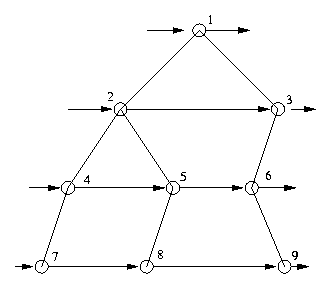
\includegraphics[width=.52\textwidth]{figuras/bfs.png}
			\caption{USACO}
		\end{figure}
	\end{center}
\end{frame}

%- - - - - - - - - - - - - - - - - - - - - - - - - - - - - - - - - SLIDE -
\begin{frame}
\frametitle{Complete Search}
\begin{block}{Busca em Largura}
\includefile{c++}{codes}{pseudobfs.cpp}
\end{block}
\end{frame}

%- - - - - - - - - - - - - - - - - - - - - - - - - - - - - - - - - SLIDE -
\begin{frame}
\frametitle{Complete Search}
\begin{block}{Busca em largura}
\begin{itemize}
	\bitem Chamada de busca em largura porque percorre uma linha inteira (a largura) da árvore de candidatos antes de passar para a próxima linha.
	\bitem Primeiro visita a raiz, então todos os nós no nível 1, depois todos no nível 2, ...
\end{itemize}
\end{block}
\pause
\begin{block}{Busca em largura -- Complexidade}
\begin{itemize}
	\bitem Complexidade de tempo é a mesma da busca em profundidade.
	\bitem Consumo de espaço proporcional ao número de candidatos.
	\begin{itemize}
		\bitem Sejam $c$ o número de escolhas para cada decisão, e $k$ o número de decisões que devem ser feitas.
		\bitem Existem $c^k$ possíveis candidatos que vão estar na fila para o próximo passo.
	\end{itemize}
\end{itemize}
\end{block}
\end{frame}

%- - - - - - - - - - - - - - - - - - - - - - - - - - - - - - - - - SLIDE -
\begin{frame}
\frametitle{Complete Search}
\begin{block}{Busca em aprofundamento iterativo}
\begin{itemize}	\bitem \emph{Depth First with Iterative Deepening} (ID)
	\bitem Alternativa a busca em largura
	\bitem São executadas sequencialmente $D$ buscas em profundidade
	\bitem Cada busca pode ir um nível além da busca anterior
	\bitem Simula uma busca em largura, complexidade de tempo pior mas gasta menos espaço
\end{itemize}
\end{block}
\end{frame}

%- - - - - - - - - - - - - - - - - - - - - - - - - - - - - - - - - SLIDE -
\begin{frame}
\frametitle{Complete Search}
\begin{block}{Busca em aprofundamento iterativo}
\includefile{c++}{codes}{pseudoid.cpp}
\end{block}
\end{frame}

%- - - - - - - - - - - - - - - - - - - - - - - - - - - - - - - - - SLIDE -
\begin{frame}
\frametitle{Complete Search}
\begin{block}{Busca em aprofundamento iterativo -- Complexidade}

\begin{itemize}
	\bitem Complexidade de espaço é a mesma da busca em profundidade;
	\bitem Complexidade de tempo pior:
	\begin{itemize}
		\bitem Busca em profundidade parando na profundidade $k$ leva $O(c^k)$
		\bitem Seja $d$ o número máximo de decisões (profundidade máxima), o tempo gasto será $c^0 + c^1 + c^2 + c^3 + ... + c^d$
	\end{itemize}
	\bitem Sempre que há pelo menos duas escolhas a serem tomadas, a busca em aprofundamento iterativo
	não gasta mais que o dobro de tempo que a busca em largura teria gasto.
\end{itemize}	

\end{block}
\end{frame}

%- - - - - - - - - - - - - - - - - - - - - - - - - - - - - - - - - SLIDE -
\begin{frame}
\frametitle{Complete Search}
\begin{block}{Quando usar?}
\begin{table}
    \begin{tabular}{|p{2.5cm}|l|l|p{5cm}|}
        \hline
        Busca                    & Tempo    & Espaço    & Quando usar                                                                                                                \\ \hline
        Profundidade             & $O(c^k)$ & $O(k)$    & a) De qualquer maneira vai olhar todos os estados, b) sabe o nível que a resposta está, ou c) não está procurando a menor resposta. \\ \hline
        Largura                  & $O(c^d)$ & $O(c^d)$  & a) Sabe que a resposta fica perto do topo da árvore, ou b) está procurando a menor resposta.                                     \\ \hline
        Aprofundamento Iterativo & $O(c^d)$ & $O(d)$    & Quer fazer uma busca em largura, não tem espaço e pode gastar um pouco mais de tempo.                                       \\
        \hline
    \end{tabular}
\end{table}
\end{block}
\end{frame}

\subsection{Hora de resolver alguns problemas..}

%- - - - - - - - - - - - - - - - - - - - - - - - - - - - - - - - - SLIDE -
\begin{frame}
\frametitle{Complete Search}
\begin{block}{The Clocks [IOI 94]}
\begin{itemize}
	\bitem Existem 9 relógios em um \emph{grid} $3\ x\ 3$; que podem estar mostrando um dos seguintes horários: 12:00, 3:00, 6:00 ou 9:00.
	\bitem Objetivo: Fazer com que todos mostrem 12:00.
	\bitem 9 comandos podem ser usados para manipular os relógios
	\begin{itemize}
		\bitem Cada comando rotaciona um subconjunto de relógios 90 graus no sentido horário. 
	\end{itemize}
	\bitem Qual a menor sequência de comandos que faz com que todos os relógios mostrem 12:00.
\end{itemize}
\end{block}
\pause
\begin{block}{}
\begin{itemize}
	\bitem Solução mais óbvia: fazer movimentos 
	\bitem 
\end{itemize}
\end{block}

%A group of nine clocks inhabits a 3 x 3 grid; each is set to 12:00, 3:00, 6:00, or 9:00. Your goal is to manipulate them all to read 12:00. Unfortunately, the only way you can manipulate the clocks is by one of nine different types of move, each one of which rotates a certain subset of the clocks 90 degrees clockwise.
%
%Find the shortest sequence of moves which returns all the clocks to 12:00.
%
%The ``obvious'' thing to do is a recursive solution, which checks to see if there is a solution of 1 move, 2 moves, etc. until it finds a solution. This would take 9k time, where k is the number of moves. Since k might be fairly large, this is not going to run with reasonable time constraints.
%
%Note that the order of the moves does not matter. This reduces the time down to k9 , which isn't enough of an improvement.
%
%However, since doing each move 4 times is the same as doing it no times, you know that no move will be done more than 3 times. Thus, there are only 49 possibilities, which is only 262,072, which, given the rule of thumb for run-time of more than 10,000,000 operations in a second, should work in time. The brute-force solution, given this insight, is perfectly adequate.
\end{frame}

%- - - - - - - - - - - - - - - - - - - - - - - - - - - - - - - - - SLIDE -
\begin{frame}
\frametitle{Complete Search}
\begin{block}{UVa 725 -- Division}
%	Encontrar dois numeros de 5 dígitos tais que, abcde / fghij = N
%	cada digito de 0-9 deve aparecer exatamente uma vez, 2  <= N <= 79
%Solução: 
%	testar todos os fghij
%	abcde = fghij*N
%	verifica restrição de uso dos digitos
\end{block}
\end{frame}

%- - - - - - - - - - - - - - - - - - - - - - - - - - - - - - - - - SLIDE -
\begin{frame}
\frametitle{Complete Search}
\begin{block}{Superprime Rib [USACO 1994 Final Round, adapted]}
%
%A number is called superprime if it is prime and every number obtained by chopping some number of digits from the right side of the decimal expansion is prime. For example, 233 is a superprime, because 233, 23, and 2 are all prime. Print a list of all the superprime numbers of length n, for n <= 9. The number 1 is not a prime.
%
%For this problem, use depth first search, since all the answers are going to be at the nth level (the bottom level) of the search.
\end{block}
\end{frame}

%- - - - - - - - - - - - - - - - - - - - - - - - - - - - - - - - - SLIDE -
\begin{frame}
\frametitle{Complete Search}
\begin{block}{Betsy's Tour [USACO 1995 Qualifying Round]}
%A square township has been partitioned into n 2 square plots. The Farm is located in the upper left plot and the Market is located in the lower left plot. Betsy takes a tour of the township going from Farm to Market by walking through every plot exactly once. Write a program that will count how many unique tours Betsy can take in going from Farm to Market for any value of n <= 6.
%
%Since the number of solutions is required, the entire tree must be searched, even if one solution is found quickly. So it doesn't matter from a time perspective whether DFS or BFS is used. Since DFS takes less space, it is the search of choice for this problem.
\end{block}
\end{frame}

%- - - - - - - - - - - - - - - - - - - - - - - - - - - - - - - - - SLIDE -
\begin{frame}
\frametitle{Complete Search}
\begin{block}{UVa 11742 -- Social Constraints}
%	0 < n <= 8 amigos vão ao cinema
%	vão se sentar na primeira fileira, com n assentos consecutivos
%	Existem 0 <= m <= 20 restrições, (a,b,c) indicando que a e b devem estar sentados no máximo a c assentos de distancia
%	De quantas formas eles podem se sentar?
%Solução
%	testar as n! permutações
%	verifica se a permutação satisfaz todas as restrições
\end{block}
\end{frame}

%- - - - - - - - - - - - - - - - - - - - - - - - - - - - - - - - - SLIDE -
\begin{frame}
\frametitle{Complete Search}
\begin{block}{UVa 12346 - Water Gate Management}
%	uma barragem tem 1 <= n <= 20 portões que deixam a água passar quando necessário, cada portão tem uma taxa que determina quanta água ele é capaz de deixar passar por segundo e um custo de abertura.
%	Sua tarefa é controlar a abertura dos portões de modo que a agua possa fluir a uma taxa de x unidades por segundo e o custo total de abertura seja minimo.
%Solução
%	testar todos os 2^n subconjuntos de portões que podem ser abertos
%	para cada subconjunto
%		verifica se a taxa passando é maior ou igual a taxa desejada
%			em caso positivo, verifique se o custo é menor que o menor custo encontrado ate agora
\end{block}
\end{frame}

%- - - - - - - - - - - - - - - - - - - - - - - - - - - - - - - - - SLIDE -
\begin{frame}
\frametitle{Complete Search}
\begin{block}{Party Lamps [IOI 98]}
%You are given N lamps and four switches. The first switch toggles all lamps, the second the even lamps, the third the odd lamps, and last switch toggles lamps 1, 4, 7, 10, ... .
%
%Given the number of lamps, N, the number of button presses made (up to 10,000), and the state of some of the lamps (e.g., lamp 7 is off), output all the possible states the lamps could be in.
%
%Naively, for each button press, you have to try 4 possibilities, for a total of 410000 (about 106020 ), which means there's no way you could do complete search (this particular algorithm would exploit recursion).
%
%Noticing that the order of the button presses does not matter gets this number down to about 100004 (about 1016 ), still too big to completely search (but certainly closer by a factor of over 106000 ).
%
%However, pressing a button twice is the same as pressing the button no times, so all you really have to check is pressing each button either 0 or 1 times. That's only 24 = 16 possibilities, surely a number of iterations solvable within the time limit.
\end{block}
\end{frame}

%- - - - - - - - - - - - - - - - - - - - - - - - - - - - - - - - - SLIDE -
\begin{frame}
\frametitle{Complete Search}
\begin{block}{Addition Chains}
%An addition chain is a sequence of integers such that the first number is 1, and every subsequent number is the sum of some two (not necessarily unique) numbers that appear in the list before it. For example, 1 2 3 5 is such a chain, as 2 is 1+1, 3 is 2+1, and 5 is 2+3. Find the minimum length chain that ends with a given number.
%
%Analysis: Depth-first search with iterative deepening works well here, as DFS has a tendency to first try 1 2 3 4 5 ... n, which is really bad and the queue grows too large very quickly for BFS.
\end{block}
\end{frame}

%- - - - - - - - - - - - - - - - - - - - - - - - - - - - - - - - - SLIDE -
\begin{frame}
\frametitle{Complete Search}
\begin{block}{Dicas}
\begin{itemize}[<+->]
	\bitem Podar o quanto antes
	\bitem Aproveitar simetrias
	\bitem Pré-cálculo
%	\bitem Inverter o problema (?)
	\bitem Otimizar código
	\bitem Usar um algoritmo/estrutura de dados melhor
\end{itemize}
\end{block}
\end{frame}

%- - - - - - - - - - - - - - - - - - - - - - - - - - - - - - - - - SLIDE -
\begin{frame}
\frametitle{Leituras Recomendadas}

\begin{block}{}
\begin{itemize}
\scriptsize
	\bitem \url{http://community.topcoder.com/tc?module=Static&d1=tutorials&d2=recursionPt1}
	\bitem \url{http://community.topcoder.com/tc?module=Static&d1=tutorials&d2=recursionPt2}
	\bitem \url{http://www.inf.ufg.br/~paulocosta/tap/material/bt1.pdf}
	\bitem \url{http://www.inf.ufg.br/~paulocosta/tap/material/bt2.pdf}
%	\bitem \url{http://www.inf.ufg.br/~paulocosta/tap/material/bt3.pdf} % MITM
	\bitem \url{http://www.comp.nus.edu.sg/~stevenha/visualization/recursion.html}
\end{itemize}
\end{block}

\end{frame}
